\PassOptionsToPackage{quiet}{fontspec}
\documentclass[12pt,a4paper,UTF8]{article}
\usepackage{thesis} % 格式控制
\usepackage{indentfirst} 
\setlength{\parindent}{2em} % 控制首行缩进  
\addtolength{\parskip}{3pt} % 控制段落距离  
\onehalfspacing % 1.5倍行距  
\graphicspath{{./figures/}} % 指定图片所在文件夹  


\classname{智能控制技术}  % 设置课程名称
\expname{HW01 专家控制}
\makepagestyle{\printexpname}{\printclassname ~实验报告}

\begin{document}
\maketitlepage{\printexpname}{教7 304}{PhilFan}{19260817}{\today}{刘山} %封面页 

\maketoc    %目录页
\section{实验目的和要求}
如图所示为车载倒立摆系统,一辆小车在水平轨道上移动,小车上有一个可绕固定点转动的倒立摆。控制小车在水平方向的移动可使摆杆维持直立不倒,这和手掌移动可使直立木棒不倒的现象类似。

忽略车轮与地面的摩擦力等阻力,可推导出车载倒立摆的动力学方程如下:

\begin{align}
\begin{cases}
(M + m) \ddot{x} + m l (\ddot{\theta} \cos \theta + ml \dot{\theta}^2 \sin \theta) = F \\
ml^2 \ddot{\theta} + ml \ddot{x} \cos \theta - mgl \sin \theta = 0
\end{cases}    
\end{align}



其中的参数如表所示:


增量型离散PID控制算法如下:

\begin{align*}
   F(k) = F(k-1) + K \left[ K_p \Delta \theta (k) + \frac{T}{T_i} \theta (k) + \frac{T}{T_d} (\Delta \theta (k) - \Delta \theta (k-1)) \right] 
\end{align*}


其中 $T$ 为采样时间,$\Delta \theta (k) = \theta (k) - \theta (k-1)$

若 $F_m = 25$,取 $T = 0.0001s$,$K_p = 200$,$K_i = 3$,$K_d = 10$

设计 $0 < \theta_1 < \theta_2 < \theta_m$,$0 < K_s < 1 < K_b$


在离散PID控制基础上,采用专家PID控制方案,规则如下:


\begin{itemize}

\item 1. 若 $|\theta(k)| \geq \theta_m$ 时,$F(k) = \text{sgn}(\theta) F_m$

\item 2. 若 $\theta_2 \leq |\theta(k)| < \theta_m$ 时,
    \begin{itemize}
        \item 若 $\theta(k) \Delta \theta(k) > 0$ 时,$K = K_b$
        \item 若 $\theta(k) \Delta \theta(k) < 0$ 时,
            \begin{itemize}
                \item 若 $\Delta \theta(k) \Delta \theta(k-1) > 0$ 时,$K = 1$
                \item 若 $\Delta \theta(k) \Delta \theta(k-1) < 0$ 时,$K = K_b$
            \end{itemize}
    \end{itemize}

\item 3. 若 $\theta_1 \leq |\theta(k)| < \theta_2$ 时,
    \begin{itemize}
        \item 若 $\theta(k) \Delta \theta(k) > 0$ 时,$K = 1$
        \item 若 $\theta(k) \Delta \theta(k) < 0$ 时,
            \begin{itemize}
                \item 若 $\Delta \theta(k) \Delta \theta(k-1) > 0$ 时,$K = K_s$
                \item 若 $\Delta \theta(k) \Delta \theta(k-1) < 0$ 时,$K = 1$
            \end{itemize}
    \end{itemize}

\item 4. 若 $|\theta(k)| < \theta_1$ 时,$K = 1$
    
\end{itemize}


若小车和摆杆静止,摆杆与垂直向上方向的初始夹角 $\theta(0) = \frac{\pi}{4} \text{ rad}$,请:


\begin{problem}
给出上述专家PID控制方案的合适参数 $\theta_1, \theta_2, \theta_m$ 和 $K_s, K_b$,通过调节 $F$ 使倒立摆的摆杆夹角 $\theta$ 恢复并维持在期望值($\theta_d = 0$),在 matlab 中进行仿真,给出位移 $x$、夹角 $\theta$ 和水平力 $F$ 的变化曲线,并比较专家PID控制与常规PID控制的结果(可尝试参数 $\theta_1 = 0.1, \theta_2 = 0.3, \theta_m = 0.5$ 和 $K_s = 1, K_b = 1.3$)。
\end{problem}

\begin{problem}
针对不同的初始夹角 $\theta(0)$,给出专家PID控制的结果。(可能需要调整相关参数 $\theta_1, \theta_2, \theta_m$ 和 $K_s, K_b$)
\end{problem}

\section{问题分析}

经过搜索和阅读题目,我认为本题可以分三个步骤来完成

\begin{enumerate}
    \item \textbf{建立小车倒立摆的物理模型}
    \item \textbf{建立普通PID和专家PID的控制器}
    \item \textbf{优化参数}
\end{enumerate}

对于第一个步骤,由于普通的状态空间模型不能表达非线性模型,所以这里我们采用了S-function进行表达

普通PID使用了Matlab中自带的PID模块。

专家PID则使用题干中的控制策略,使用S-function构造一个输入是$\theta$,状态变量是$[\theta, \frac{d\theta}{dt}, \theta_{last}, error_{sum}, error_{last}]$,输出变量是$F$的控制器 

对于调参来讲,我们先使用题目中推荐的参数进行测试,开始使用了观察法,比较普通PID和专家PID的控制效果;
之后我参考机器学习中的损失函数,设计了基于MSE和最小超调$theta$值的$cost\ funtion$,并设计了\texttt{critic} 评分器,用来比较PID和专家PID的实验结果.

同时,我的代码结构也比较规范,增加了详细的注释和说明,并添加了版本管理系统。

\clearpage % 换页
\section{算法设计}


\subsection{S-function学习}

S-function模块位于Simulink/User-Defined Functions模块库中,是使S-function图形化的模板工具,用于为S-function创建一个定值的对话框和图标。


\begin{itemize}
    \item \textbf{S-function name}:填入S-function的函数名称,这样就建立了S-function模块与M文件形式的S-function之间的对应关系;
    \item \textbf{S-function parameters}:填入S-function需要输入的外部参数的名称,如果有多个变量,则变量中间用逗号隔开,如a,b,c;
    \item \textbf{S-function modules}:仅当S-function是用C语言编写并用MEX工具编译的C-MEX文件时,才需要填写该参数;
\end{itemize}

\textbf{直接馈通}

如果输出函数(\texttt{mdlOutputs}或\texttt{flag==3})是输入\texttt{u}的函数,即,如果输入\texttt{u}在\texttt{mdlOutputs}中被访问,则存在直接馈通。例如:
\[ y = k \cdot u \]

\textbf{采样时间与偏移量}

采样时间是按照固定格式成对指定的:\texttt{[采样时间 偏移时间]}。

\begin{table}[h]
    \centering
    \begin{tabular}{|c|c|}
        \hline
        采样时间表示 & 意义 \\
        \hline
        \texttt{[0 0]} & 连续采样时间 \\
        \hline
        \texttt{[-1 0]} & 继承S-function输入信号或父层模型的采样时间 \\
        \hline
        \texttt{[0.5 0.1]} & 离散采样时间,从0.1s开始每0.5s采样一次 \\
        \hline
    \end{tabular}
    \caption{采样时间与偏移量}
\end{table}

\textbf{函数分析}

S-function包括主函数和6个功能子函数,包括\texttt{mdlInitializeSizes}(初始化)、\texttt{mdlDerivatives}(连续状态微分)、\texttt{mdlUpdate}(离散状态更新)、\texttt{mdlOutputs}(模块输出)、\texttt{mdlGetTimeOfNextVarHit}(计算下次采样时刻)和\texttt{mdlTerminate}(仿真结束)。

在S-function仿真过程中,利用\texttt{switch-case}语句,根据不同阶段对应的\texttt{flag}值(仿真流程标志向量)来调用S-function的不同子函数,以完成对S-function模块仿真流程的控制。

\subsection{Mask}

如果我们不想每次修改S-function的参数都要打开S-function的编辑窗口,我们可以使用Mask功能。

\textbf{第一步:增加Mask}

\begin{figure}[h]
    \centering
    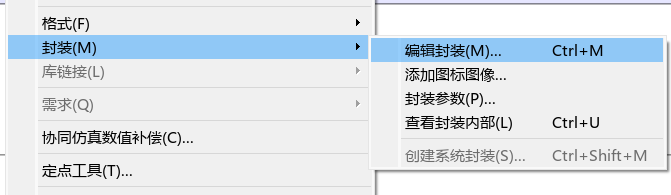
\includegraphics[width=0.6\textwidth]{20241203115042.png}
    \caption{增加Mask}
\end{figure}

\begin{figure}[h]
    \centering
    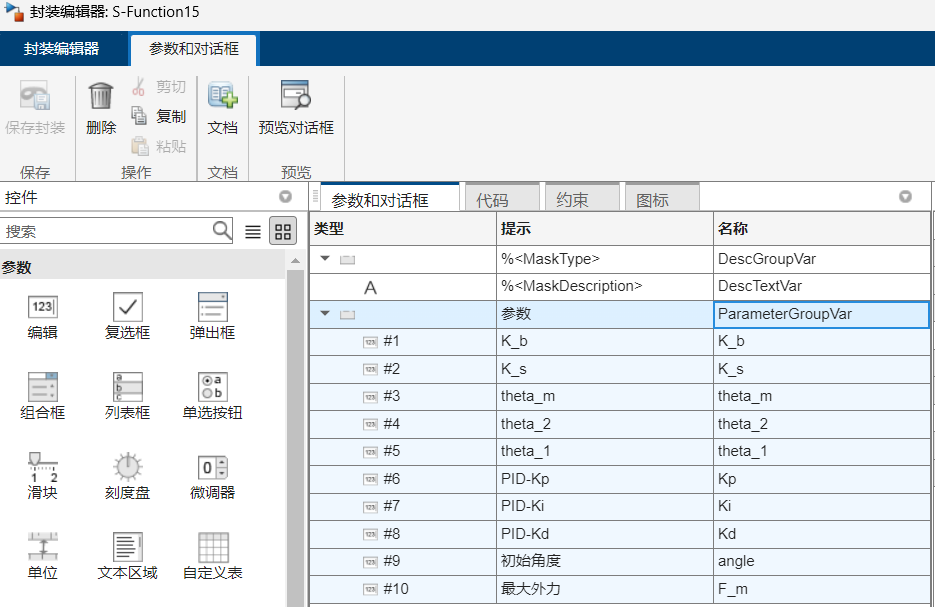
\includegraphics[width=0.6\textwidth]{20241203115132.png}
    \caption{点击添加封装}
\end{figure}

提示框可以随便写,但是名称需要和代码中的变量名称对齐。

\textbf{第二步:在S-function初始化当中加入Mask参数}

\begin{lstlisting}
function [sys,x0,str,ts,simStateCompliance] = expert_control(t,x,u,flag,K_b,K_s,theta_m,theta_2,theta_1,Kp,Ki,Kd,angle,F_m) %这里需要加上需要的参数
    switch flag
        case 0
            [sys,x0,str,ts,simStateCompliance]=mdlInitializeSizes(angle); % 注意这里要写上需要的参数
        case 1
            sys=mdlDerivatives(t,x,u);
        case 2
            sys=mdlUpdate(t,x,u,K_b,K_s,theta_m,theta_2,theta_1,Kp,Ki,Kd,F_m); % 注意这里要写上需要的参数
        case 3
            sys=mdlOutputs(t,x,u);
        case 4
            sys=mdlGetTimeOfNextVarHit(t,x,u);
        case 9
            sys=mdlTerminate(t,x,u);
        otherwise
            DAStudio.error('Simulink:blocks:unhandledFlag', num2str(flag));
    end

%% 子函数定义部分
function [sys,x0,str,ts,simStateCompliance]=mdlInitializeSizes(angle) % 注意这里要写上需要的参数
\end{lstlisting}

\textbf{第三步:在s-function的模块参数中,添加需要预置的参数}

在参数这一行把需要的参数填进去,按照顺序来
\begin{figure}[!htbp]
\centering
\begin{minipage}[b]{0.45\linewidth}
    \centering
     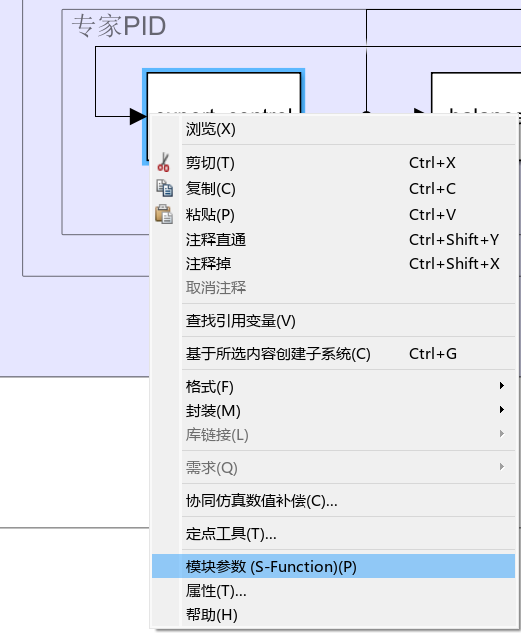
\includegraphics[width=0.6\textwidth]{20241203114952.png}
\caption{添加需要预置的参数}
     
\end{minipage}%
\begin{minipage}[b]{0.45\linewidth}
    \centering
   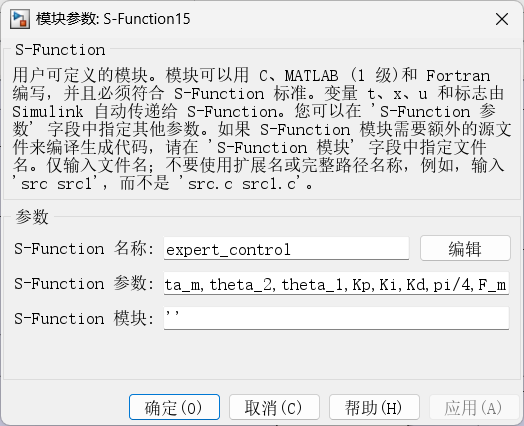
\includegraphics[width=0.8\textwidth]{20241203115502.png}
\caption{参数设置}
\end{minipage}
\end{figure}




\clearpage
\subsection{普通PID建模}

对于小车,我们使用s-function进行建模,这里使用$x,\dot{x},\theta,\dot{\theta}$作为状态变量。

核心的S-function函数为:

\begin{lstlisting}[language=Matlab]
function sys=mdlDerivatives(t,x,u)
    % 系统参数定义
    m = 0.5;                          % 摆杆质量(kg)
    M = 1;                            % 小车质量(kg)
    l = 0.5;                          % 摆杆半长(m)
    g = 9.8;                          % 重力加速度(m/s^2)
    % 计算状态导数
    dx1 = x(2);                       % 小车位置的导数
    dx3 = x(4);                       % 摆杆角度的导数
    dx2 = (u - m^2*l^2*x(4)^2*sin(x(3)) - m*g*sin(x(3))*cos(x(3))) / (M + m*sin(x(3))^2);  % 小车速度的导数
    dx4 = ( m*g*l*sin(x(3)) - m*l*cos(x(3))*dx2) / (m*l^2); % 摆杆角速度的导数,注意这里可以使用已经计算过的简化表达
    sys = [dx1; dx2; dx3; dx4];       % 返回导数向量
\end{lstlisting}


对于PID算法,我直接采用了Simulink中自带的PID模块使用。需要设计的参数是,采样时间$t = 0.0001$,$K_P=200$,$K_i=0.001$,$K_d=10$。得到了如图\ref{F-1},\ref{x-1},\ref{theta-1}的曲线。可以发现,只采用单环PID控制,$\theta$收敛,但是x发散,这和朴素的理解也是相符的。

\begin{figure}[!htbp]
    \centering
    \begin{minipage}[b]{0.6\linewidth}
        \centering
        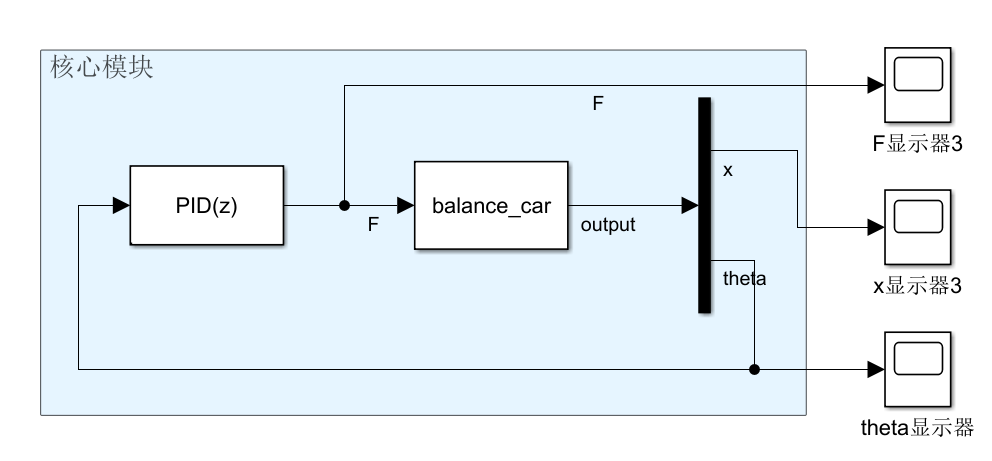
\includegraphics[width=0.9\linewidth]{figures/struc.png}
\caption{核心模块的结构}
         
    \end{minipage}%
    \begin{minipage}[b]{0.35\linewidth}
        \centering
        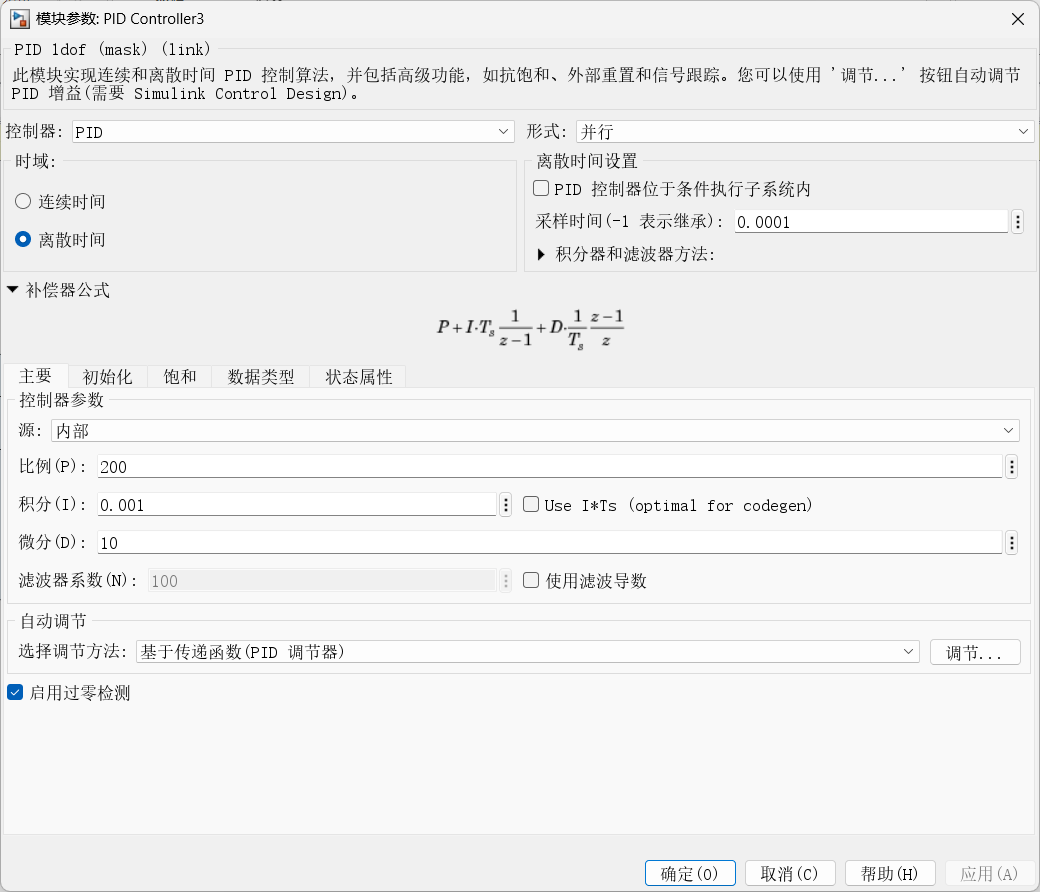
\includegraphics[width=0.8\linewidth]{figures/set1.png}
\caption{参数设计}
         
    \end{minipage}
\end{figure}


\begin{figure}[htbp]
    \centering
    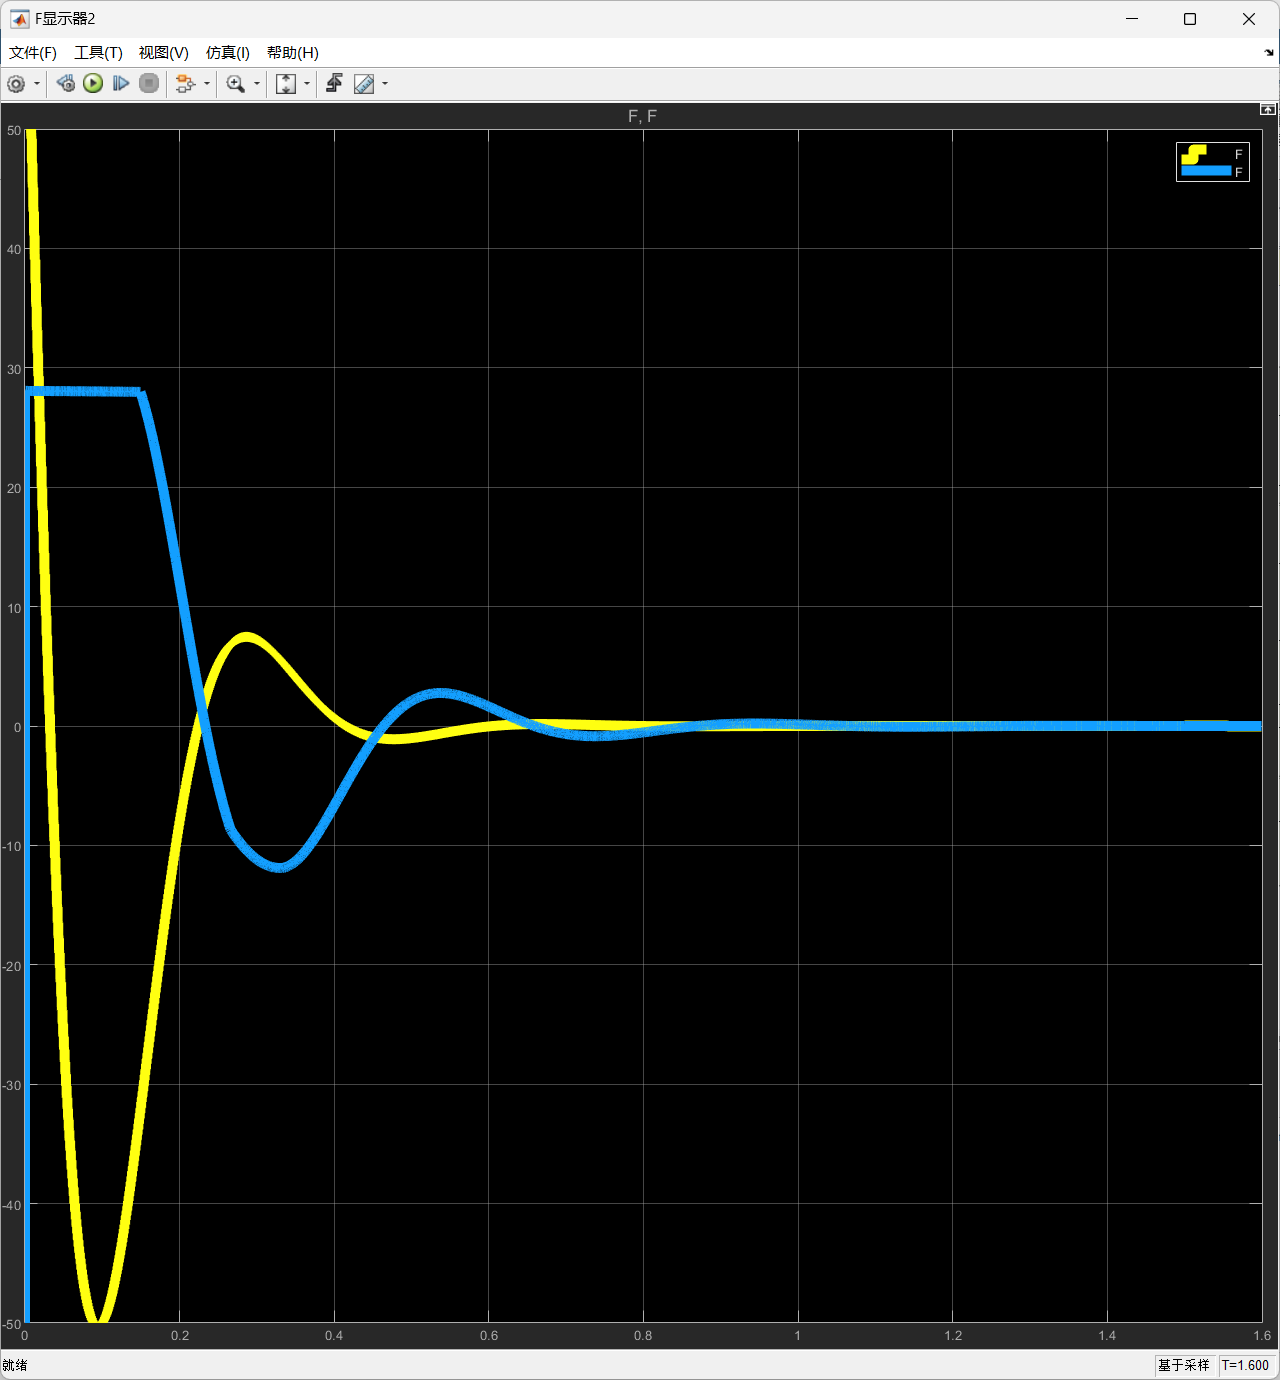
\includegraphics[width=0.8\linewidth]{figures/f.png}
    \caption{$F$的图像}
    \label{F-1}
\end{figure}

\begin{figure}[htbp]
    \centering
    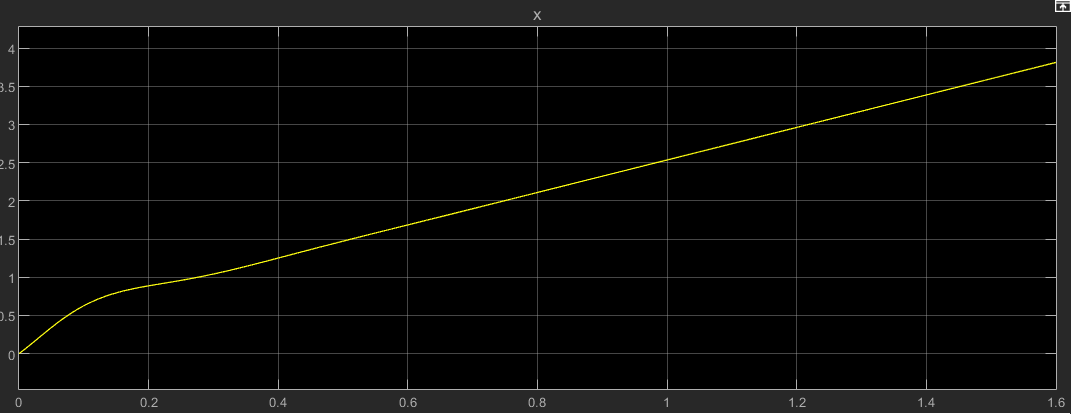
\includegraphics[width=0.8\linewidth]{figures/x.png}
    \caption{$x$的图像}
    \label{x-1}
\end{figure}

\begin{figure}[htbp]
    \centering
    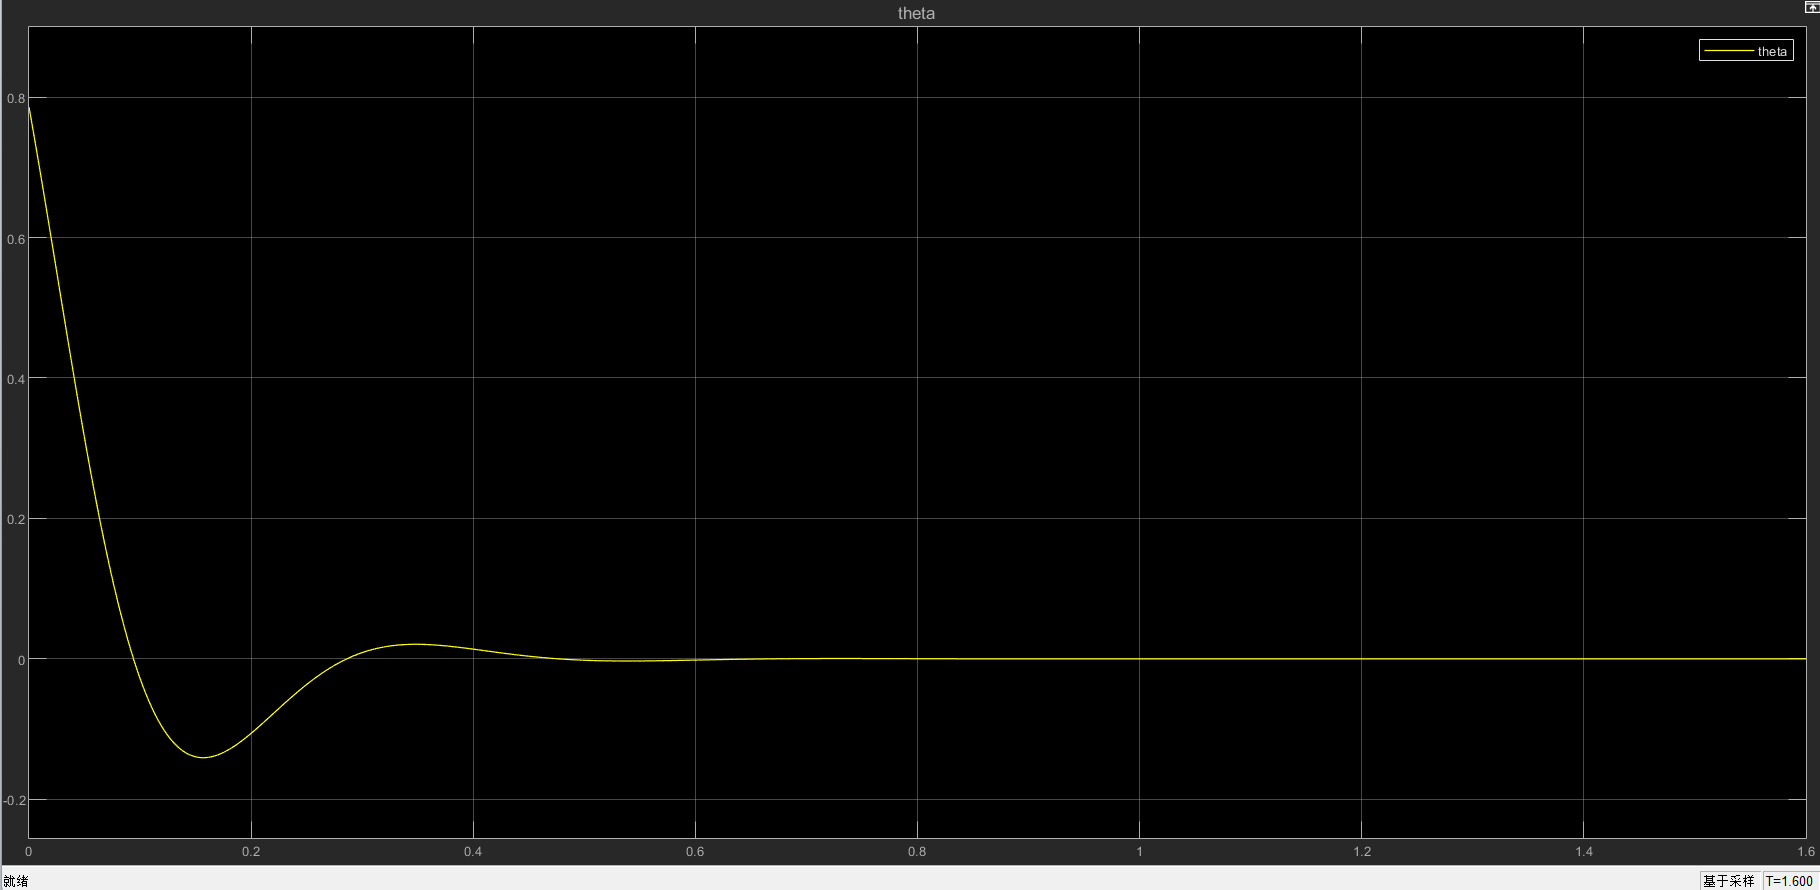
\includegraphics[width=0.8\linewidth]{figures/theta.png}
    \caption{$\theta$的图像}
    \label{theta-1}
\end{figure}

\clearpage
\subsection{专家PID策略分析}

专家PID控制策略是一种基于规则的PID控制方法,它根据被控对象的状态和变化趋势来动态调整PID控制器的参数,以达到更好的控制效果。具体来说,专家PID控制策略包括以下几个规则:

\begin{enumerate}
    \item \textbf{大角度控制规则}:
    \begin{itemize}
        \item 当角度绝对值 $|\theta(k)|$ 大于或等于最大允许角度 $\theta_m$ 时,控制器输出 $F(k)$ 为最大控制力 $F_m$,并且方向与角度 $\theta(k)$ 的符号相同。这种规则确保了在角度过大时,控制器能够迅速采取强有力的措施来纠正偏差。
    \end{itemize}
    
    \item \textbf{中角度控制规则}:
    \begin{itemize}
        \item 当角度绝对值 $|\theta(k)|$ 在 $\theta_2$ 和 $\theta_m$ 之间时,控制器根据角度的变化趋势来调整增益 $K$:
        \begin{itemize}
            \item 如果角度 $\theta(k)$ 和其变化率 $\Delta \theta(k)$ 同号(即角度在增加且变化率正,或者角度在减小且变化率负),则增益 $K$ 为基本增益 $K_b$。
            \item 如果角度 $\theta(k)$ 和其变化率 $\Delta \theta(k)$ 异号,则进一步根据变化率的符号变化来调整增益:
            \begin{itemize}
                \item 如果当前变化率 $\Delta \theta(k)$ 和前一时刻的变化率 $\Delta \theta(k-1)$ 同号,则增益 $K$ 为1。
                \item 如果当前变化率 $\Delta \theta(k)$ 和前一时刻的变化率 $\Delta \theta(k-1)$ 异号,则增益 $K$ 为基本增益 $K_b$。
            \end{itemize}
        \end{itemize}
    \end{itemize}
    
    \item \textbf{小角度控制规则}:
    \begin{itemize}
        \item 当角度绝对值 $|\theta(k)|$ 在 $\theta_1$ 和 $\theta_2$ 之间时,控制器同样根据角度的变化趋势来调整增益 $K$:
        \begin{itemize}
            \item 如果角度 $\theta(k)$ 和其变化率 $\Delta \theta(k)$ 同号,则增益 $K$ 为1。
            \item 如果角度 $\theta(k)$ 和其变化率 $\Delta \theta(k)$ 异号,则进一步根据变化率的符号变化来调整增益:
            \begin{itemize}
                \item 如果当前变化率 $\Delta \theta(k)$ 和前一时刻的变化率 $\Delta \theta(k-1)$ 同号,则增益 $K$ 为阻尼增益 $K_s$。
                \item 如果当前变化率 $\Delta \theta(k)$ 和前一时刻的变化率 $\Delta \theta(k-1)$ 异号,则增益 $K$ 为1。
            \end{itemize}
        \end{itemize}
    \end{itemize}
    
    \item \textbf{小角度控制规则}:
    \begin{itemize}
        \item 当角度绝对值 $|\theta(k)|$ 小于 $\theta_1$ 时,增益 $K$ 为1。这种规则适用于角度接近目标值时,采用较小的增益以避免过度调整。
    \end{itemize}
\end{enumerate}




根据这些规则,我设计了我的专家控制S-function,核心代码如下

\begin{lstlisting}[language=Matlab,caption=专家控制核心代码]
% 专家控制规则
if abs(theta_k) >= theta_m
    % 规则1: 角度大于等于theta_m,施加最大外力
    F = sign(theta_k) * F_m;
elseif abs(theta_k) >= theta_2
    % 规则2: theta_2到theta_m区间的控制
    if theta_k * delta_theta_k > 0
        K = K_b;
    elseif theta_k * delta_theta_k < 0
        if delta_theta_k * delta_theta_k_1 > 0
            K = 1;
        elseif delta_theta_k * delta_theta_k_1 < 0
            K = K_b;
        end
    end
elseif abs(theta_k) >= theta_1
    % 规则3: theta_1到theta_2区间的控制
    if theta_k * delta_theta_k > 0
        K = 1;
    else
        if delta_theta_k * delta_theta_k_1 > 0
            K = K_s;
        elseif delta_theta_k * delta_theta_k_1 < 0
            K = 1;
        end
    end
else
    K = 1;
end

% 计算控制力
F = F + K * (Kp * delta_theta_k + (T / T_i) * theta_k + (T_d / T) * (delta_theta_k - delta_theta_k_1));
\end{lstlisting}

\clearpage
\subsection{critic评分器设计}

为了更好的量化普通PID和专家PID的调整结果,参考在《机器学习》课程中的思想,我设计了一个Critic评价函数,采用MSE($\sum u^2$)和最大化最小$\theta$($max \ \theta_{min}$)的方式。

为了权衡这两种不同的评价指标,我设计了一个cost的计算公式:

\begin{align}
cost = \alpha \cdot (ref - u)^2 + \beta \cdot abs(\theta_{min})
\end{align}

在这个critic评价体系下,我们的参数调整就变成了一个优化问题:

\begin{align}
cost^* = \mathop{arg\ min }_{u \in U} \left[\alpha \cdot (ref - u)^2 + \beta \cdot abs(\theta_{min})\right]
\end{align}

当然,这种评价方式带有了一定的归纳偏置,所以这个critic函数还有很多优化的空间。


对于critic评价器,我也是使用S-function实现的,核心代码如下:
\begin{lstlisting}[language=Matlab,caption=critic核心代码]
function sys = mdlUpdate(t, x, u)
    % 状态更新回调子函数
    % 更新最小值theta_min,保存当前theta_k与历史最小值比较
    theta_k = u;  % 当前的theta值
    theta_min = min(x(1), theta_k);  % 更新最小值
    cost_function = x(2) + u * u ;  % 使用MSE计算成本函数
    sys = [theta_min, cost_function];
end
\end{lstlisting}

\clearpage
\section{实验结果表现与分析}
根据上面的三个模块,我实现了PID和专家PID系统,并集成到了一个子系统中进行比较。

\subsection{$\theta = \frac{\pi}{4}$时}
首先来看最基础的任务

\begin{figure}[htbp]
    \centering
    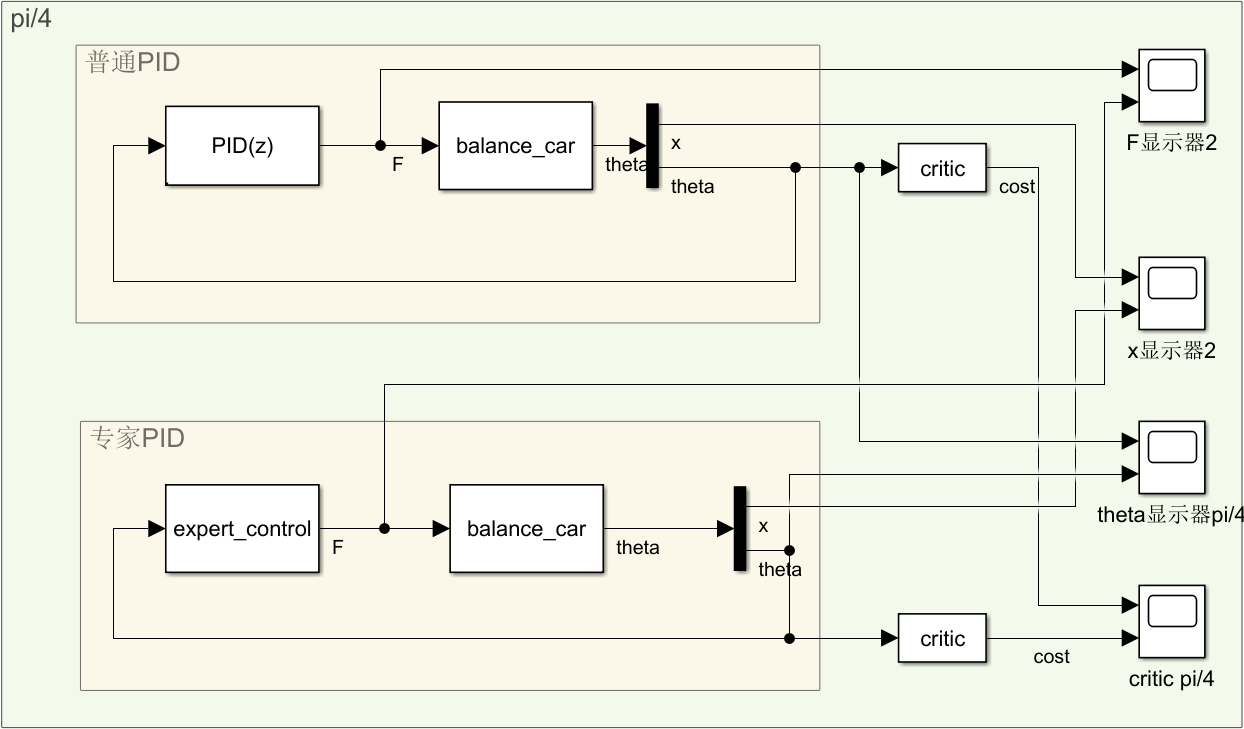
\includegraphics[width=1\linewidth]{figures/k1.png}
    \caption{$\theta = \frac{\pi}{4}$}
\end{figure}

我设置的参数如下图所示。在这样的参数下,普通PID和专家PID的cost值分别为16.0421和10.2557,在这个角度下,专家PID的效果是更为优秀的。


\begin{figure}[htbp]
    \centering
    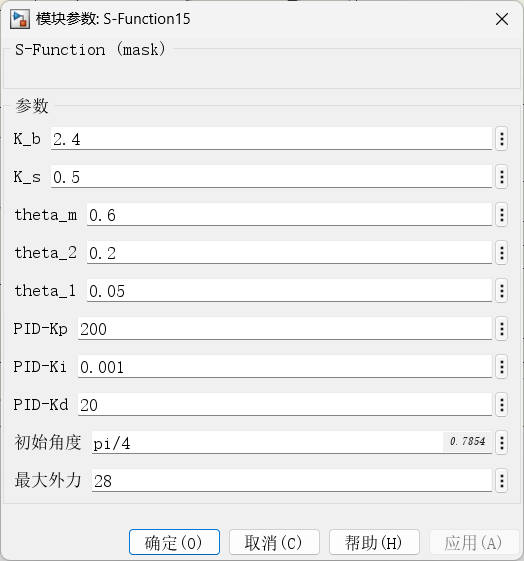
\includegraphics[width=0.4\linewidth]{figures/parameter_pi4.png}
    \caption{我的参数设置}
\end{figure}

\begin{figure}[!htbp]
    \centering
    \begin{minipage}[b]{0.45\linewidth}
        \centering
        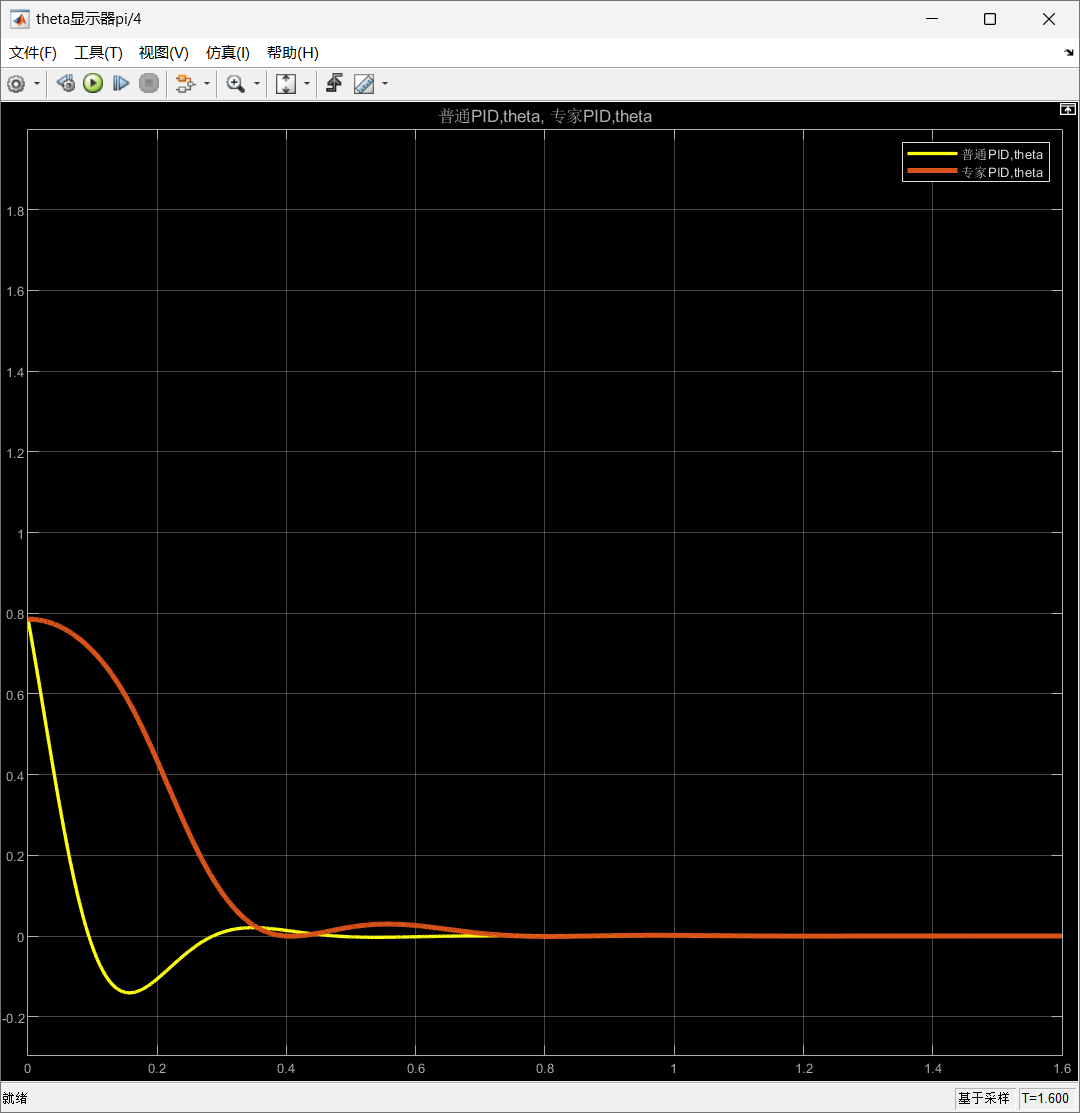
\includegraphics[width=0.9\linewidth]{figures/theta_output.png}
        \caption{theta对比图}
         
    \end{minipage}%
    \begin{minipage}[b]{0.45\linewidth}
        \centering
        \includegraphics[width=0.9\linewidth]{figures/F.png}
        \caption{F对比图}
    \end{minipage}
    
    \begin{minipage}[b]{0.45\linewidth}
        \centering
        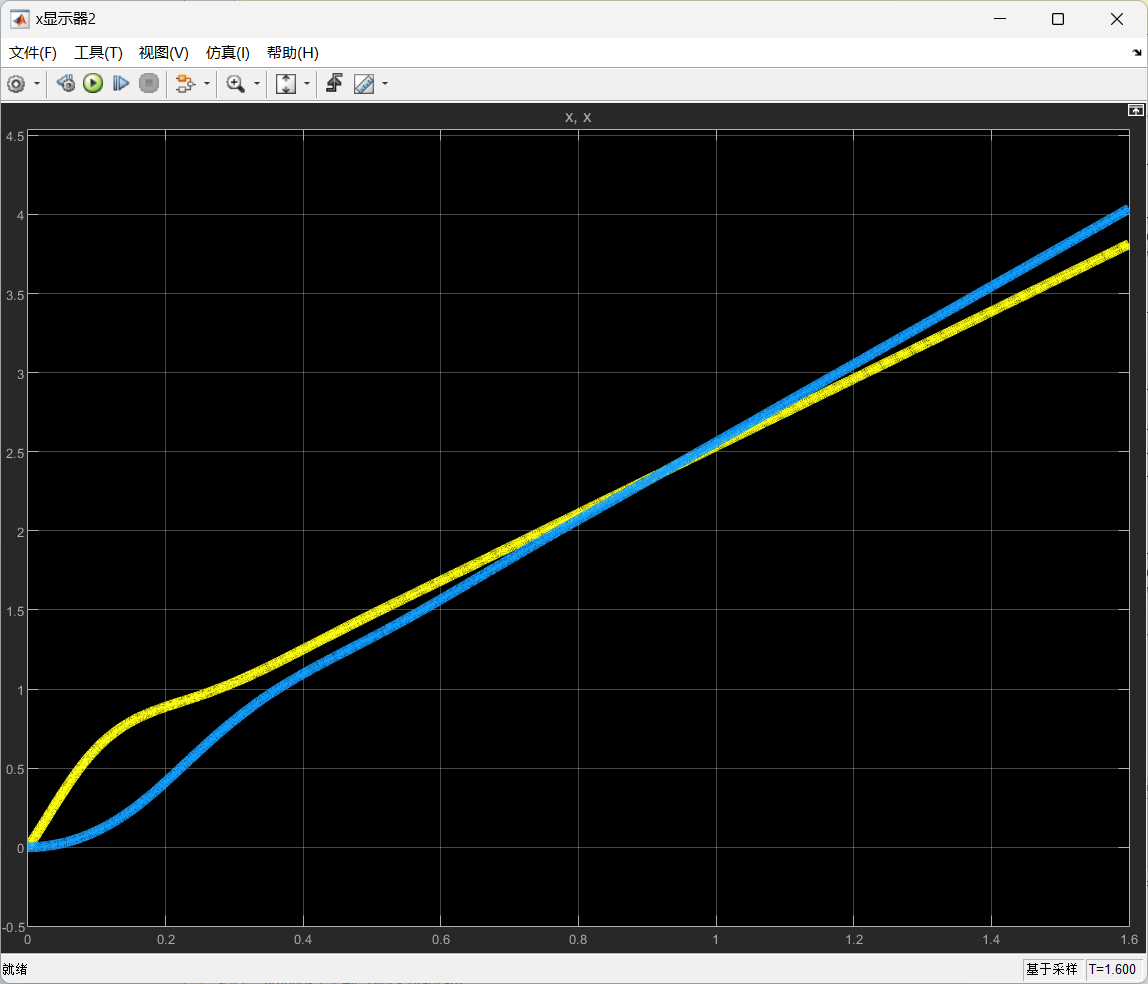
\includegraphics[width=0.9\linewidth]{figures/x_1.png}
        \caption{x对比图}
    \end{minipage}
\end{figure}


\newpage
\subsection{$\theta = \frac{\pi}{3}$时}
在$\theta = \frac{\pi}{3}$时,普通PID可以直接稳定,在调整专家PID参数后,专家PID也可以稳定。

并且在图\ref{para}所示的参属下,普通PID的cost为12.4184,专家PID的cost为12.1391。可以达到给定目标。

\begin{figure}[htbp]
    \centering
    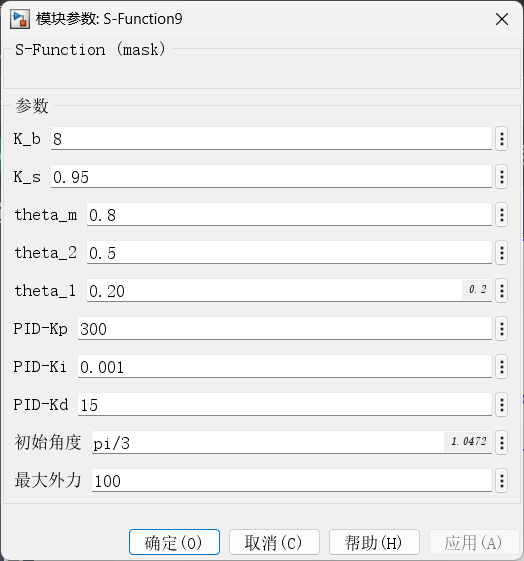
\includegraphics[width=0.3\linewidth]{figures/para.png}
    \caption{参数设置}
    \label{para}
\end{figure}


\begin{figure}[!htbp]
    \centering
    \begin{minipage}[b]{0.45\linewidth}
        \centering
        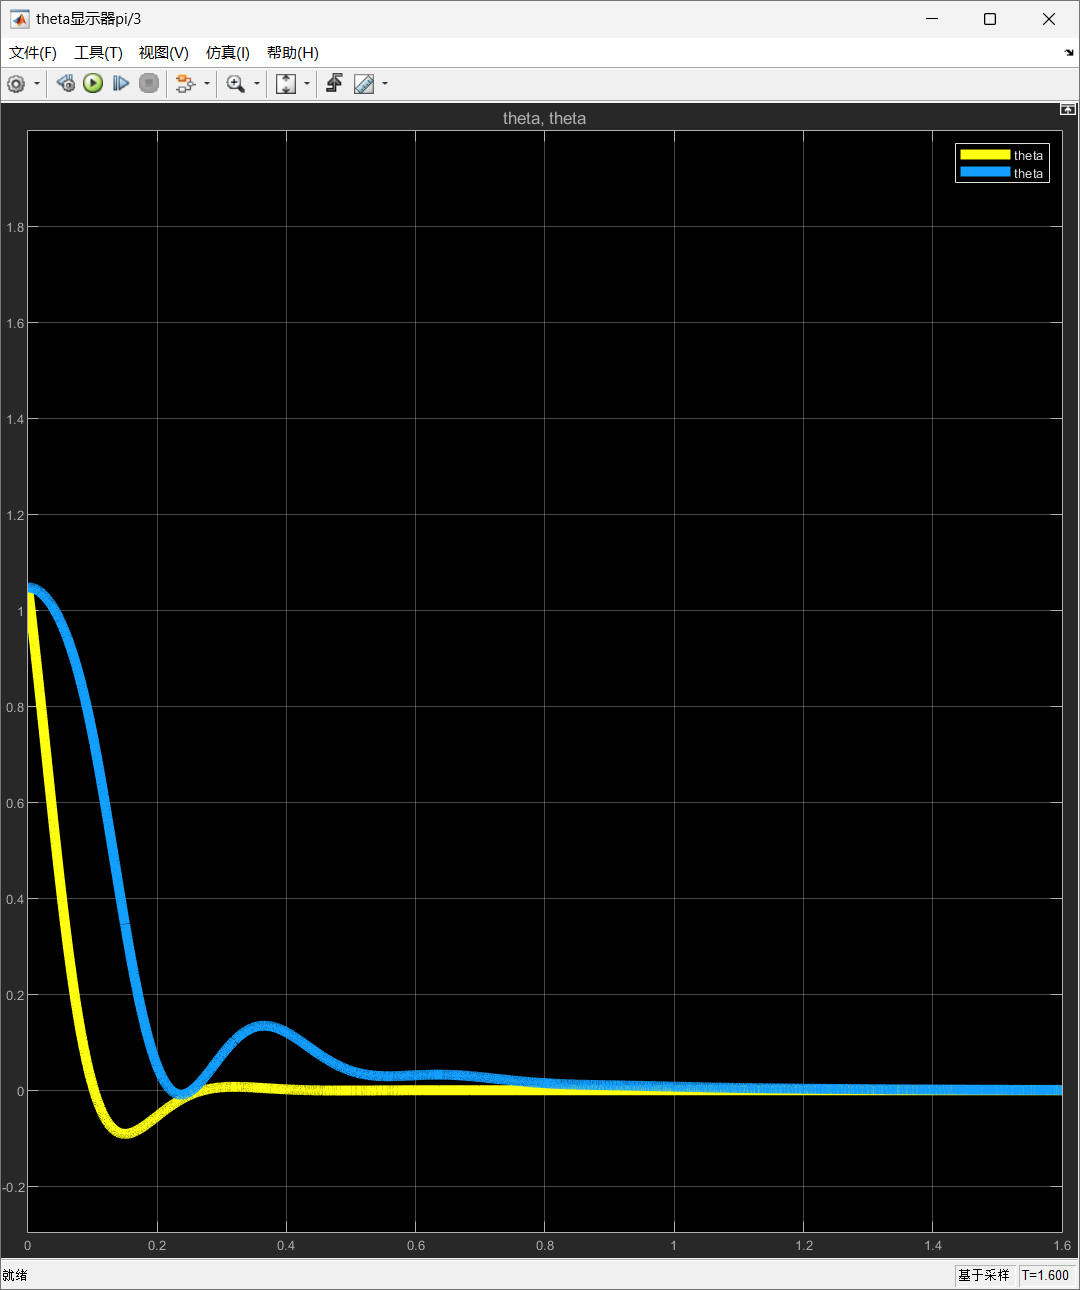
\includegraphics[width=0.7\linewidth]{figures/image.png}
        \caption{$\theta$的对比}
         
    \end{minipage}% 
    \begin{minipage}[b]{0.45\linewidth}
        \centering
        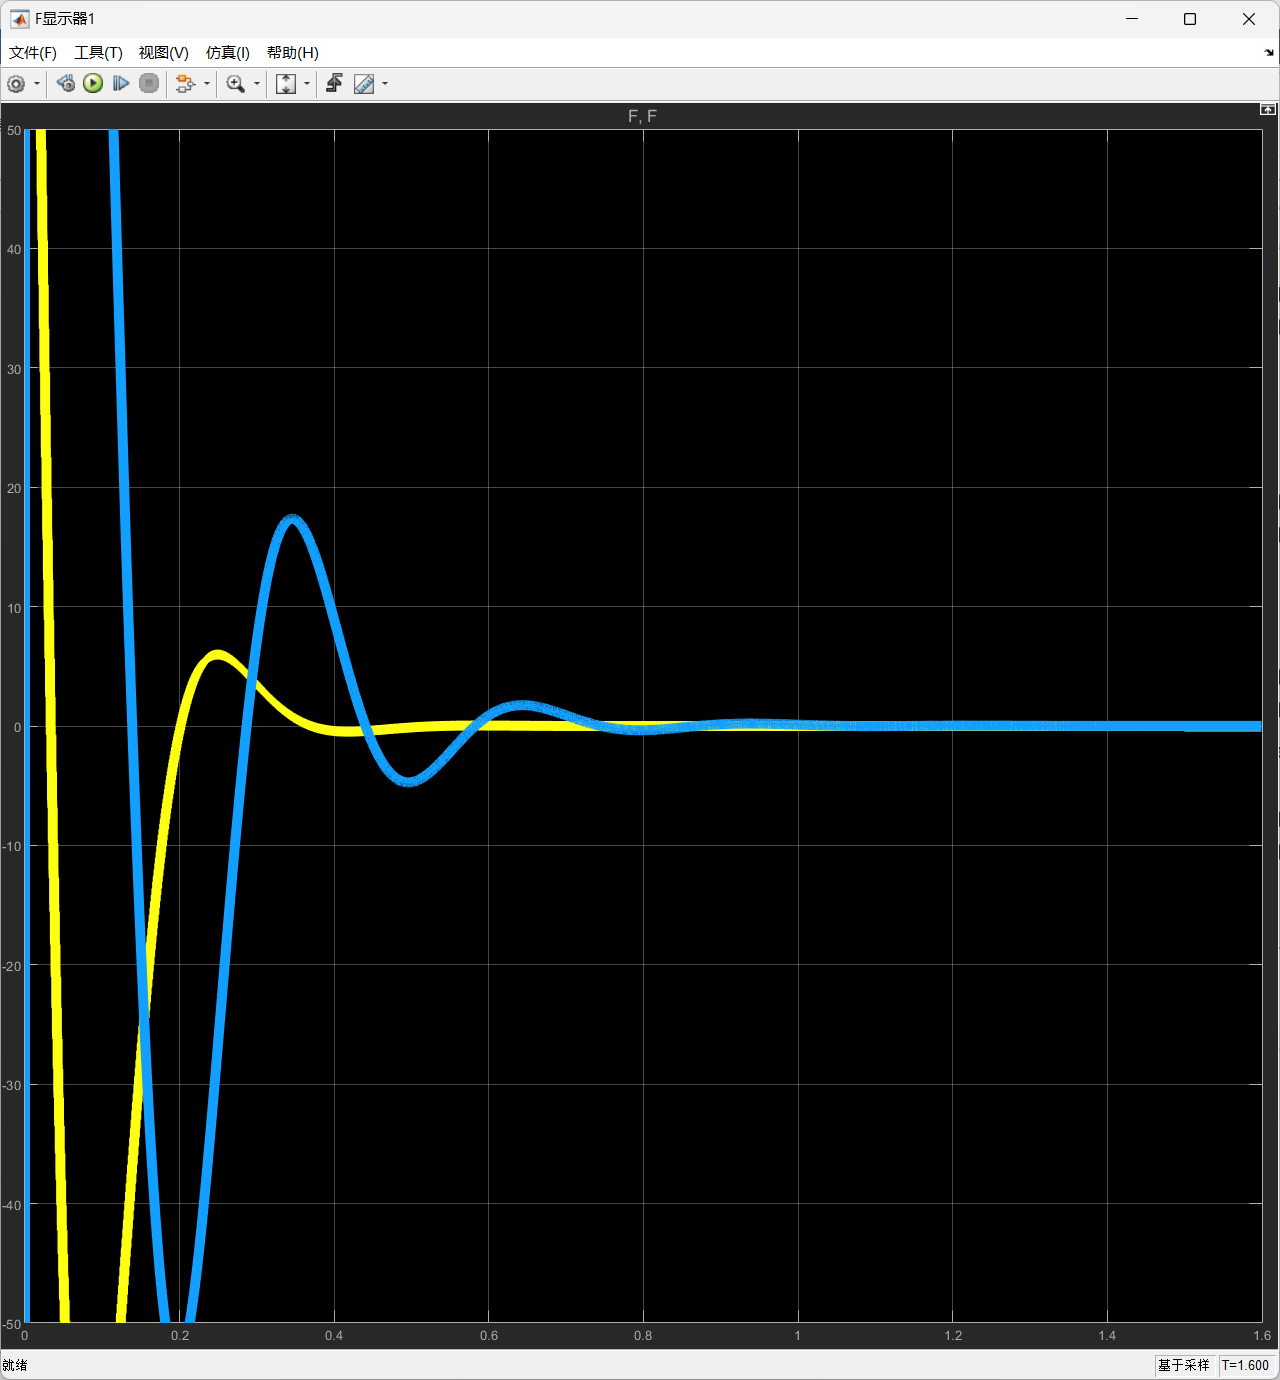
\includegraphics[width=0.7\linewidth]{figures/f_2.png}
    \caption{F对比图}
    \end{minipage}
    
    \begin{minipage}[b]{0.45\linewidth}
        \centering
        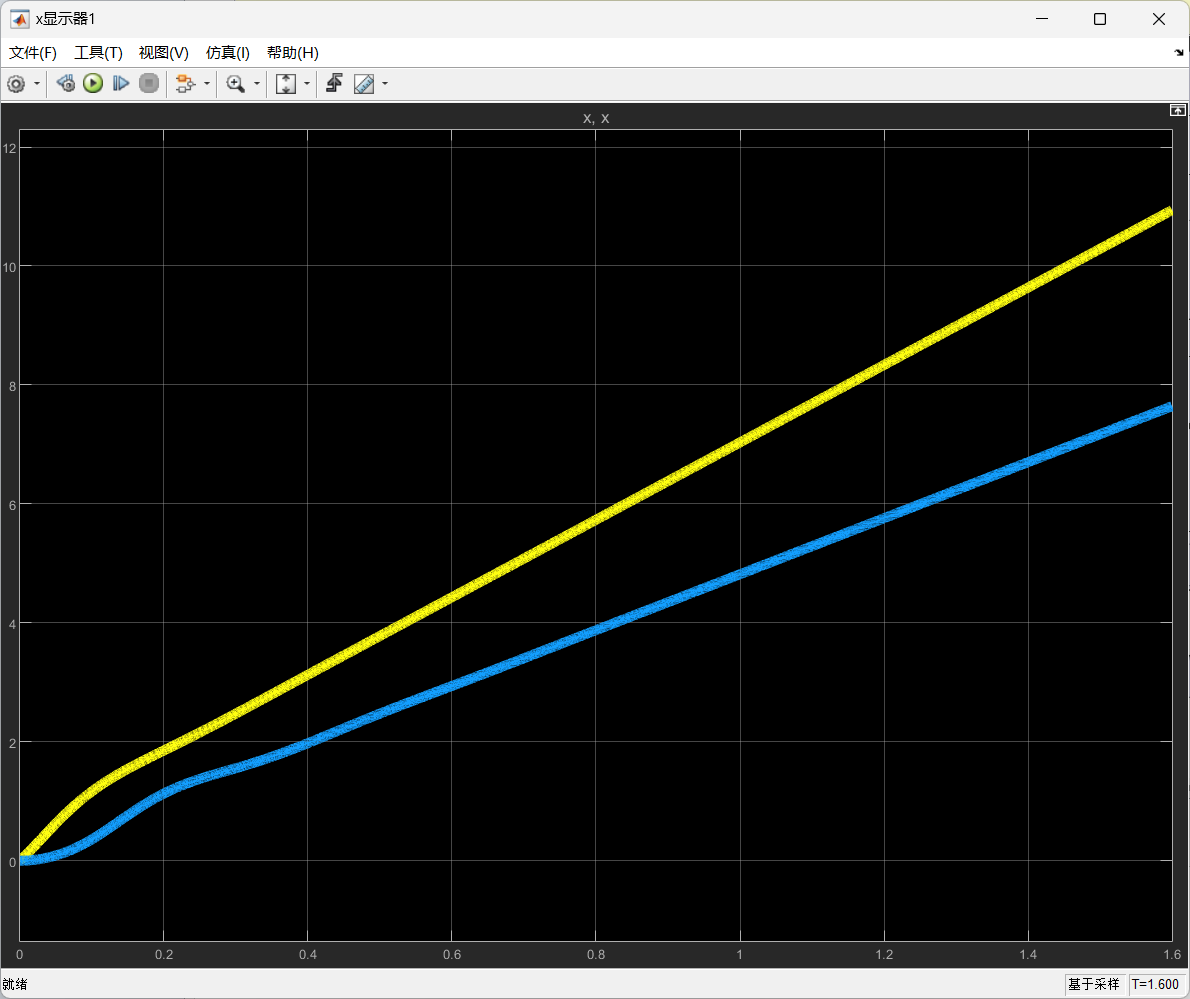
\includegraphics[width=0.8\linewidth]{figures/x_2.png}
        \caption{x的对比}
    \end{minipage}
\end{figure}


\subsection{$\theta = \frac{\pi}{6}$时}

对于$\theta= \frac{\pi}{6}$的情况,我们应该对应地减小相应参数的大小

经过调整以后,我的参数如下图所示,在这个参数设置下,普通PID的cost为6.3159,专家PID为3.3014

\begin{figure}[htbp]
    \centering
    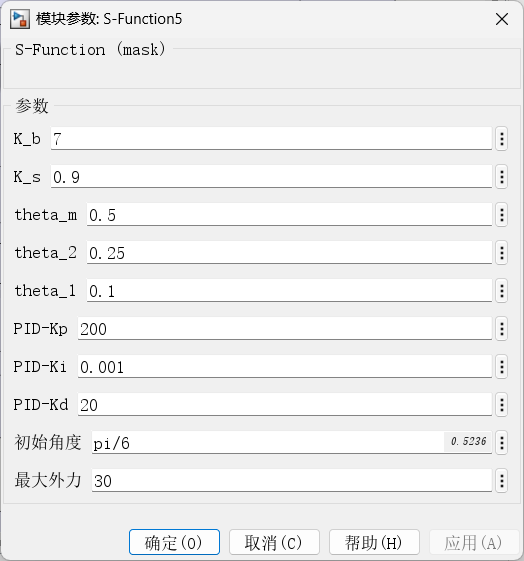
\includegraphics[width=0.3\linewidth]{figures/para_3.png}
    \caption{参数设置}
\end{figure}

\begin{figure}[!htbp]
    \centering
    \begin{minipage}[b]{0.45\linewidth}
        \centering
        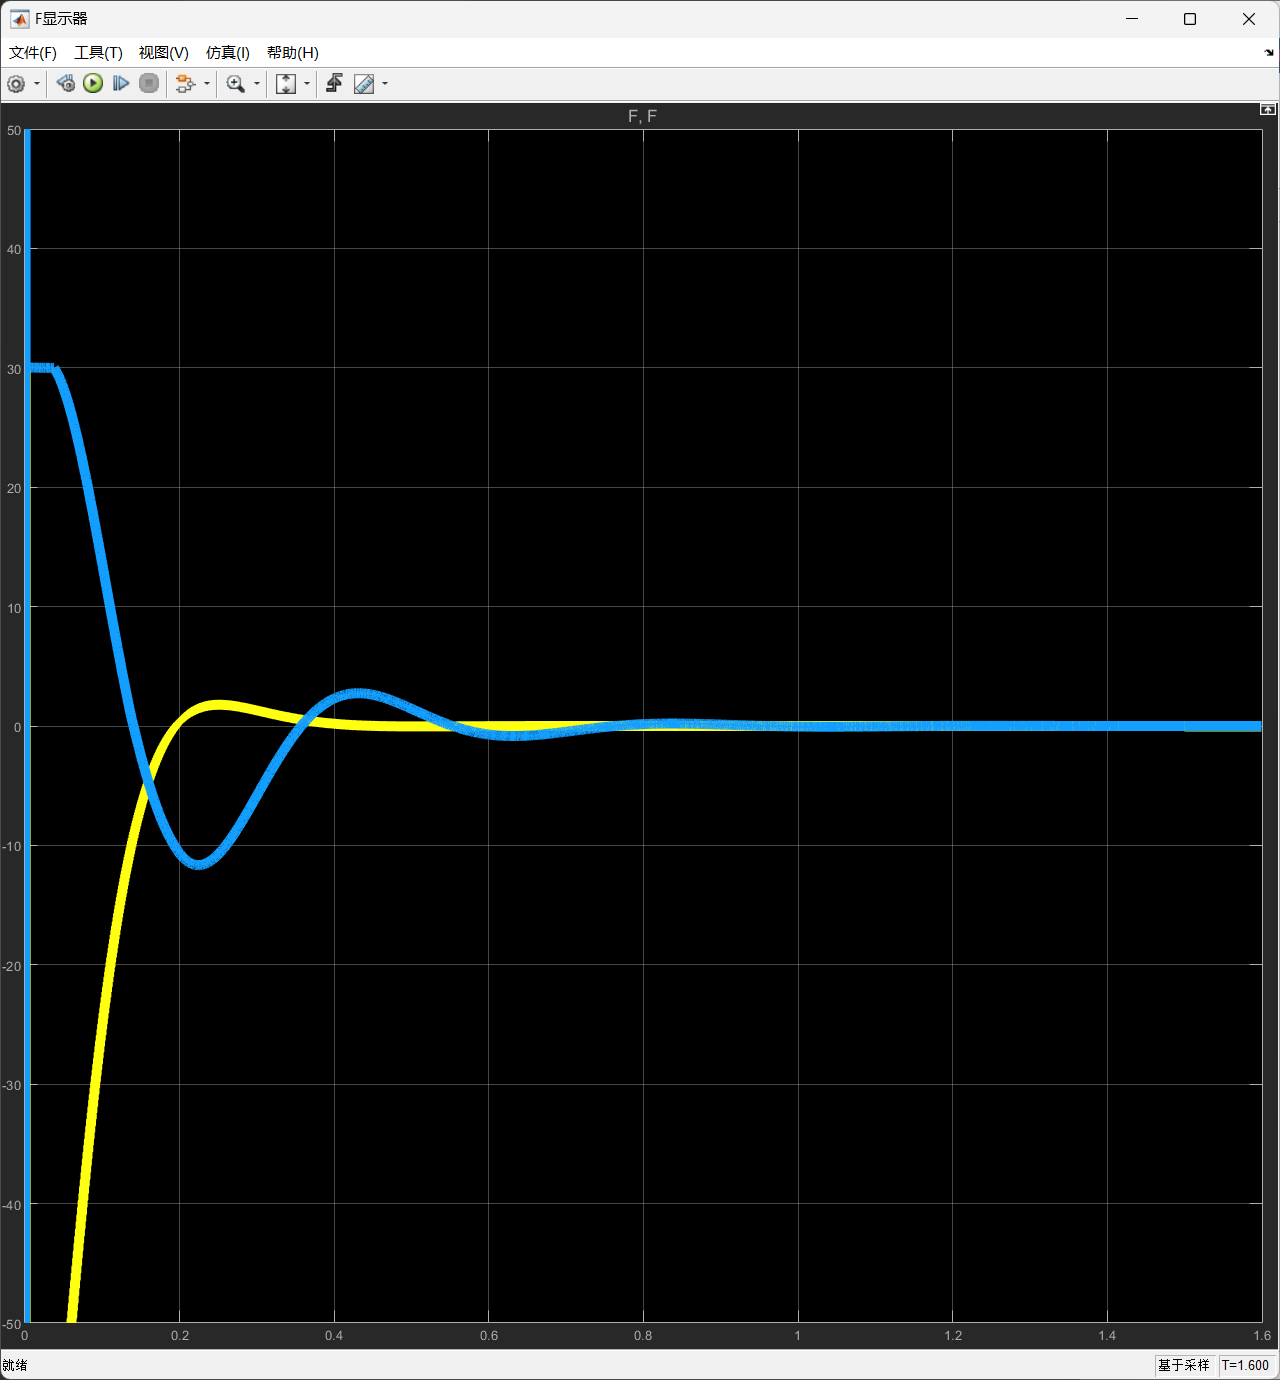
\includegraphics[width=0.5\linewidth]{figures/F_3.png}
    \caption{F结果}
    \end{minipage}
    \begin{minipage}[b]{0.45\linewidth}
        \centering
        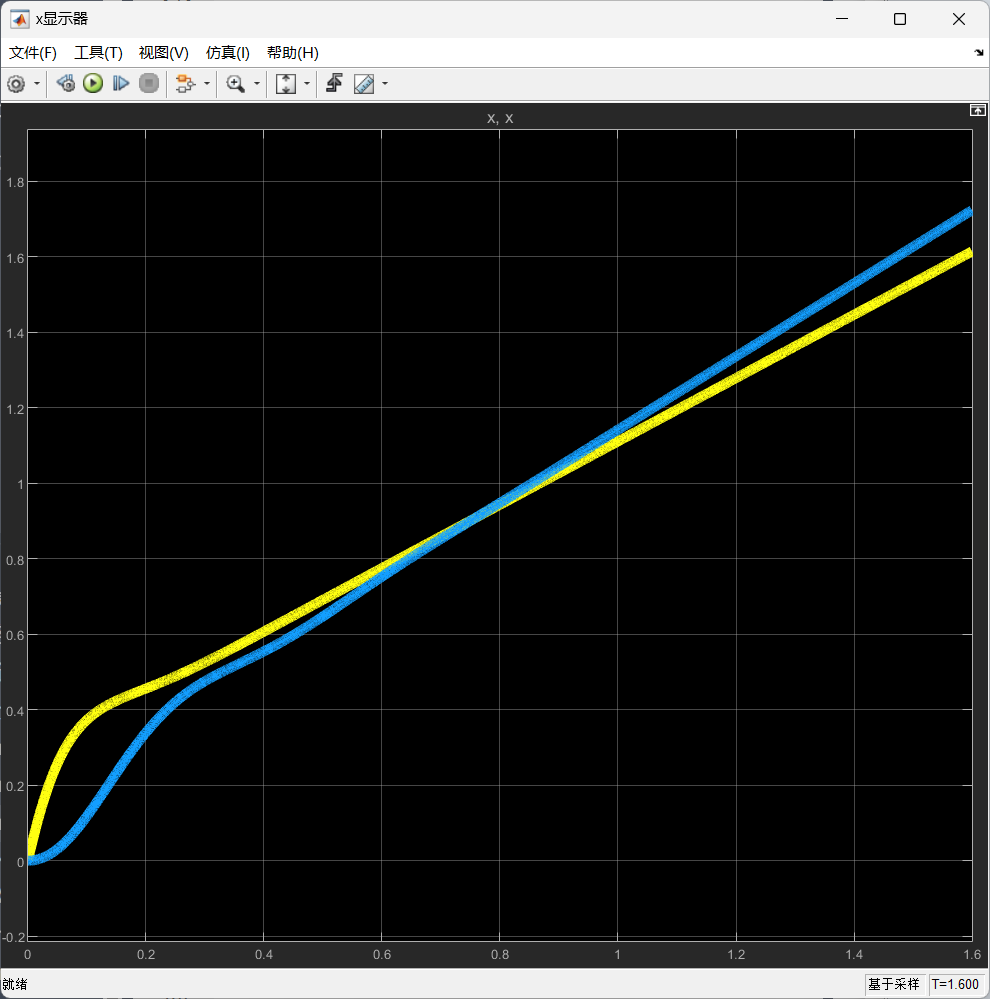
\includegraphics[width=0.6\linewidth]{figures/x_3.png}
    \caption{x对比}
    \end{minipage}
    
    \begin{minipage}[b]{0.45\linewidth}
        \centering
        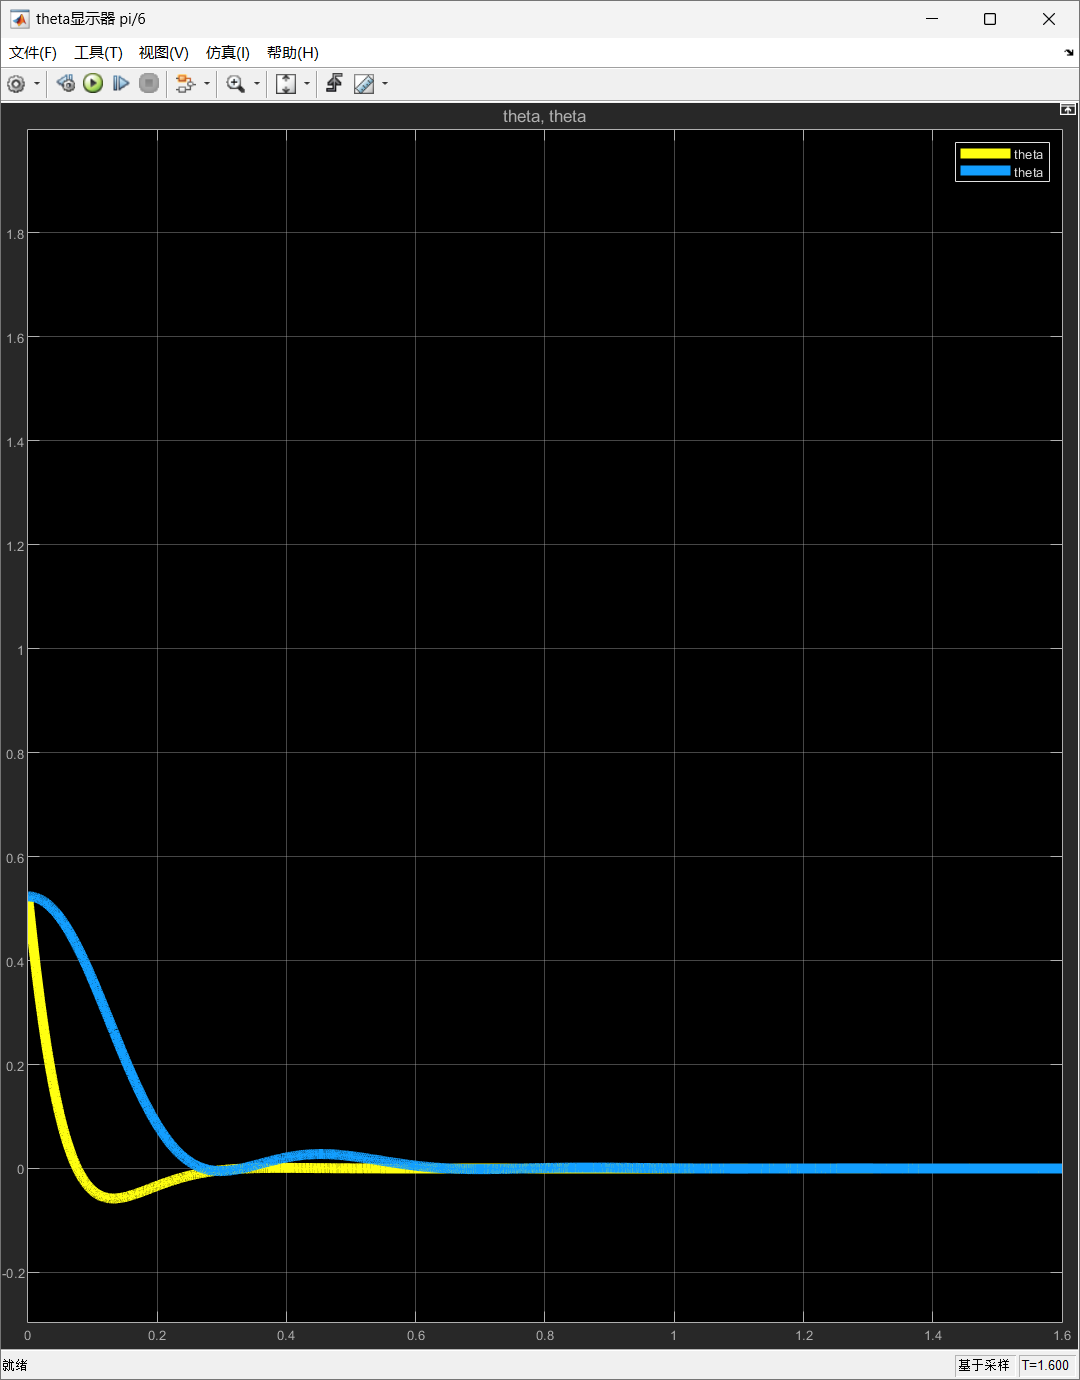
\includegraphics[width=0.7\linewidth]{figures/theta_3.png}
    \caption{$\theta$结果,蓝色为专家控制}
    \end{minipage}% 
\end{figure}

\section{实验探究与可优化方向}

总体来说,这次作业让我体会到了专家控制的整体思路和过程。在这次作业当中,我学习了s-function与mask的使用方法。并使用了一种critic函数来定量评价指标。

我认为还可以在以下几个方面做出优化:

\begin{itemize}
    \item 增加根据critic函数自动优化求解的方法
    \item 增加3D animation界面,可视化呈现
    \item 自动化地调节PID参数,或者通过可视化地调节;目前调节参数只能调完一次重新运行,效率比较低
    \item 完善系统文档
\end{itemize}


\clearpage
\appendix

\section{附录1:文档结构}

\begin{lstlisting}
.
├── expert_control.prj     # 项目文件
├── exp.slx                # 专家控制系统模型
├── expert_control.m       # 专家控制器主程序
├── critic.m              # 系统评价器
├── balance_car.m         # 倒立摆小车模型
└── README.md             # 项目说明文档
\end{lstlisting}



\section{附录2:源程序代码}
\subsection{balance\_car.m}
\section{附录3:版本更新记录}
\begin{lstlisting}[language=Matlab]
% Date: 2024-11-30
% Author: PhilFan 

% 倒立摆小车物理系统的S-function文件
% 输入参数:
%   t - 当前时间
%   x - 状态变量
%   u - 输入变量
%   flag - 仿真标志
%   angle - 初始角度
% 输出参数:
%   sys - 返回值
%   x0 - 初始状态
%   str - 保留参数
%   ts - 采样时间
%   simStateCompliance - 仿真状态


function [sys,x0,str,ts,simStateCompliance] = balance_car(t,x,u,flag,angle)
    switch flag,
        case 0,
            [sys,x0,str,ts,simStateCompliance]=mdlInitializeSizes(angle);
        case 1,
            sys=mdlDerivatives(t,x,u);
        case 2,
            sys=mdlUpdate(t,x,u);
        case 3,
            sys=mdlOutputs(t,x,u);
        case 4,
            sys=mdlGetTimeOfNextVarHit(t,x,u);
        case 9,
            sys=mdlTerminate(t,x,u);
        otherwise
            DAStudio.error('Simulink:blocks:unhandledFlag', num2str(flag));
    end

%% 子函数定义部分

function [sys,x0,str,ts,simStateCompliance]=mdlInitializeSizes(angle)
    % 初始化函数
    % 功能: 初始化系统的状态、输入输出维度等基本参数
    % 当flag=0时被调用

    sizes = simsizes;                 % 生成sizes数据结构
    sizes.NumContStates  = 4;         % 连续状态数量: 4个
    sizes.NumDiscStates  = 0;         % 离散状态数量: 0个
    sizes.NumOutputs     = 2;         % 输出数量: 2个
    sizes.NumInputs      = 1;         % 输入数量: 1个
    sizes.DirFeedthrough = 0;         % 是否存在直接馈通: 否
    sizes.NumSampleTimes = 1;         % 采样时间个数: 1个

    sys = simsizes(sizes);            % 返回初始化信息
    x0  = [0 0 angle 0];             % 设置初始状态值
    str = [];                         % 保留参数置空
    ts  = [0 0];                      % 设置采样时间
    simStateCompliance = 'UnknownSimState';

    % 状态变量说明:
    % x(1) = x     - 小车位置
    % x(2) = dx/dt - 小车速度
    % x(3) = θ     - 摆杆角度
    % x(4) = dθ/dt - 摆杆角速度

function sys=mdlDerivatives(t,x,u)
    % 系统连续状态方程
    % 功能: 计算系统状态导数
    % 当flag=1时被调用

    % 系统参数定义
    m = 0.5;                          % 摆杆质量(kg)
    M = 1;                            % 小车质量(kg)
    l = 0.5;                          % 摆杆半长(m)
    g = 9.8;                          % 重力加速度(m/s^2)

    % 计算状态导数
    dx1 = x(2);                       % 小车位置的导数
    dx3 = x(4);                       % 摆杆角度的导数
    dx2 = (u - m^2*l^2*x(4)^2*sin(x(3)) - m*g*sin(x(3))*cos(x(3))) / (M + m*sin(x(3))^2);  % 小车速度的导数
    dx4 = ( m*g*l*sin(x(3)) - m*l*cos(x(3))*dx2) / (m*l^2);                                 % 摆杆角速度的导数

    sys = [dx1; dx2; dx3; dx4];       % 返回导数向量

function sys=mdlUpdate(t,x,u)
    % 离散状态更新函数
    % 功能: 更新系统的离散状态
    % 当flag=2时被调用
    sys = [];                         % 本系统无离散状态

function sys=mdlOutputs(t,x,u)
    % 输出方程
    % 功能: 计算系统输出
    % 当flag=3时被调用
    sys = [x(1);x(3)];               % 输出小车位置和摆杆角度

function sys=mdlGetTimeOfNextVarHit(t,x,u)
    % 变采样时间计算函数
    % 功能: 计算下一个采样时间点
    % 当使用变采样时间时被调用
    sampleTime = 1;                   % 设置采样间隔为1秒
    sys = t + sampleTime;             % 计算下一个采样时间点

function sys=mdlTerminate(t,x,u)
    % 终止函数
    % 功能: 完成仿真结束时的必要工作
    % 当flag=9时被调用
    sys = [];                         % 清空系统
\end{lstlisting}

\subsection{critic.m}

\begin{lstlisting}[language=Matlab]
% Date: 2024-12-03
% Author: PhilFan 

% 评价网络定义
% 输入参数:
%   t - 当前时间
%   x - 状态变量 [theta_min, cost_function]
%   u - 输入变量 theta (摆杆角度)
%   flag - 仿真标志
% 输出参数:
%   sys - 返回值
%   x0 - 初始状态
%   str - 保留参数
%   ts - 采样时间
%   simStateCompliance - 仿真状态
% 功能说明:
%   该评价网络用于评估倒立摆系统的性能
%   通过最小化超调来优化控制效果
%   cost_function基于MSE进行计算


function [sys, x0, str, ts, simStateCompliance] = critic(t, x, u, flag)
    % Critic S-Function
    % 输入:theta,目标值theta_target(无实际意义),
    % 输出:cost_function(基于最小theta的最大化)

    switch flag
        case 0
            [sys, x0, str, ts, simStateCompliance] = mdlInitializeSizes();
        case 1
            sys = mdlDerivatives(t, x, u);
        case 2
            sys = mdlUpdate(t, x, u);
        case 3
            sys = mdlOutputs(t, x, u);
        case 4
            sys = mdlGetTimeOfNextVarHit(t, x, u);
        case 9
            sys = mdlTerminate(t, x, u);
        otherwise
            DAStudio.error('Simulink:blocks:unhandledFlag', num2str(flag));
    end

    %% 子函数定义
    function [sys, x0, str, ts, simStateCompliance] = mdlInitializeSizes()
        % 初始化回调子函数
        
        sizes = simsizes;
        sizes.NumContStates = 0;   % 连续状态数
        sizes.NumDiscStates = 2;   % 离散状态数:[theta_min, cost_function]
        sizes.NumOutputs = 1;      % 输出个数(成本函数)
        sizes.NumInputs = 1;       % 输入个数(theta)
        sizes.DirFeedthrough = 1;  % 允许直馈通道
        sizes.NumSampleTimes = 1;  % 采样时间数
        sys = simsizes(sizes);     % 返回sizes数据结构
        x0 = [Inf, 0];             % 初始状态:[theta_min, cost_function]
        str = [];                  % 保留参数
        ts = [0 0];                % 采样时间
        simStateCompliance = 'UnknownSimState'; % 仿真状态合规性
    end

    function sys = mdlDerivatives(t, x, u)
        % 导数回调子函数(不使用,空实现)
        sys = [];
    end

    function sys = mdlUpdate(t, x, u)
        % 状态更新回调子函数
        % 更新最小值theta_min,保存当前theta_k与历史最小值比较
        theta_k = u;  % 当前的theta值
        theta_min = min(x(1), theta_k);  % 更新最小值
        cost_function = x(2) + u * u ;  % 使用MSE计算成本函数
        sys = [theta_min, cost_function];
    end

    function sys = mdlOutputs(t, x, u)
        % 输出回调子函数
        % 输出成本函数
        alpha = 100;
        beta = 0.01;
        cost = x(2);
        min = x(1);
        fi  = beta*cost + alpha * abs(min);
        sys = [fi];    % 输出成本函数
    end

    function sys = mdlGetTimeOfNextVarHit(t, x, u)
        % 计算下一个采样时间(定时采样)
        sampleTime = 1;  % 固定采样时间(1秒)
        sys = t + sampleTime;  % 下一次采样时间
    end

    function sys = mdlTerminate(t, x, u)
        % 仿真结束时的回调(输出成本函数)
        alpha = 100;
        beta = 0.01;
        %disp(['min: ', num2str(x(1))]);
        
        cost = x(2);
        min = x(1);
        fi  = beta*cost + alpha * abs(min);
        disp(['cost: ', num2str(fi)]);
        sys = [];
    end
end
\end{lstlisting}


\subsection{expert\_control.m}

\begin{lstlisting}[language=Matlab]
% Date: 2024-12-01
% Author: PhilFan 

% 倒立摆专家控制系统的S-function文件
% 输入参数:
%   t - 当前时间
%   x - 状态变量 [theta, dtheta/dt, theta_last, error_sum, error_last]
%   u - 输入变量 theta (摆杆角度)
%   flag - 仿真标志
%   K_b - 基本控制器增益
%   K_s - 切换控制器增益
%   theta_m - 最大角度阈值
%   theta_2 - 第二角度阈值
%   theta_1 - 第一角度阈值
%   Kp - PID控制器比例增益
%   Ki - PID控制器积分增益
%   Kd - PID控制器微分增益
%   angle - 初始角度
%   F_m - 最大控制力
% 输出参数:
%   sys - 返回值
%   x0 - 初始状态
%   str - 保留参数
%   ts - 采样时间
%   simStateCompliance - 仿真状态
% 功能说明:
%   该专家控制系统根据摆杆角度的不同区域,
%   自适应切换不同的控制策略(PID控制和能量控制),
%   实现倒立摆的平衡控制


function [sys,x0,str,ts,simStateCompliance] = expert_control(t,x,u,flag,K_b,K_s,theta_m,theta_2,theta_1,Kp,Ki,Kd,angle,F_m)
    % 主函数,包含四个输出:
    % sys - 包含某个子函数返回的值
    % x0 - 所有状态的初始化向量
    % str - 保留参数,总是一个空矩阵
    % ts - 返回系统采样时间
    % simStateCompliance - 仿真状态合规性
    
    switch flag
        case 0
            [sys,x0,str,ts,simStateCompliance]=mdlInitializeSizes(angle);
        case 1
            sys=mdlDerivatives(t,x,u);
        case 2
            sys=mdlUpdate(t,x,u,K_b,K_s,theta_m,theta_2,theta_1,Kp,Ki,Kd,F_m);
        case 3
            sys=mdlOutputs(t,x,u);
        case 4
            sys=mdlGetTimeOfNextVarHit(t,x,u);
        case 9
            sys=mdlTerminate(t,x,u);
        otherwise
            DAStudio.error('Simulink:blocks:unhandledFlag', num2str(flag));
    end

%% 子函数定义部分
function [sys,x0,str,ts,simStateCompliance]=mdlInitializeSizes(angle)
    % 初始化回调子函数
    % 提供状态、输入输出、采样时间数目和初始状态的值
    % 初始化阶段,标志变量flag首先被置为0,S-function首次被调用时该子函数被调用
    
    sizes = simsizes;                  % 生成sizes数据结构
    sizes.NumContStates = 0;           % 连续状态数
    sizes.NumDiscStates = 5;           % 离散状态数
    sizes.NumOutputs = 1;              % 输出个数
    sizes.NumInputs = 1;               % 输入个数
    sizes.DirFeedthrough = 1;          % 是否存在直馈通道
    sizes.NumSampleTimes = 1;          % 采样时间个数
    
    sys = simsizes(sizes);             % 返回size数据结构
    x0 = [angle 0 angle 0 0];          % 设置初始状态
    str = [];                          % 保留变量置空
    ts = [0 0];                        % 设置采样时间
    simStateCompliance = 'UnknownSimState';

function sys=mdlDerivatives(t,x,u)
    sys = [];

function sys=mdlUpdate(t,x,u,K_b,K_s,theta_m,theta_2,theta_1,Kp,Ki,Kd,F_m)
    % 状态更新回调子函数
    % 给定t、x、u计算离散状态的更新
    
    theta_k = u;
    theta_k_1 = x(1);
    delta_theta_k = theta_k - theta_k_1;
    delta_theta_k_1 = x(1)-x(2);
    F = x(5);

    % PID控制参数
    K = 1;
    T = 0.0001;
    T_i = 0.001;
    T_d = 10;

    % 专家控制规则
    if abs(theta_k) >= theta_m
        % 规则1: 角度大于等于theta_m,施加最大外力
        F = sign(theta_k) * F_m;
    elseif abs(theta_k) >= theta_2
        % 规则2: theta_2到theta_m区间的控制
        if theta_k * delta_theta_k > 0
            K = K_b;
        elseif theta_k * delta_theta_k < 0
            if delta_theta_k * delta_theta_k_1 > 0
                K = 1;
            elseif delta_theta_k * delta_theta_k_1 < 0
                K = K_b;
            end
        end
    elseif abs(theta_k) >= theta_1
        % 规则3: theta_1到theta_2区间的控制
        if theta_k * delta_theta_k > 0
            K = 1;
        else
            if delta_theta_k * delta_theta_k_1 > 0
                K = K_s;
            elseif delta_theta_k * delta_theta_k_1 < 0
                K = 1;
            end
        end
    else
        K = 1;
    end

    % 计算控制力
    F = F + K * (Kp * delta_theta_k + (T / T_i) * theta_k + (T_d / T) * (delta_theta_k - delta_theta_k_1));

    % 更新系统状态
    sys = [theta_k, theta_k_1, delta_theta_k, delta_theta_k_1, F];

function sys=mdlOutputs(t,x,u)
    % 计算输出回调函数
    % 输出当前控制力F
    sys = [x(5)];

function sys=mdlGetTimeOfNextVarHit(t,x,u)
    % 计算下一个采样时间
    % 仅在系统是变采样时间系统时调用
    sampleTime = 1;
    sys = t + sampleTime;

function sys=mdlTerminate(t,x,u)
    % 仿真结束时的回调函数
    sys = [];
\end{lstlisting}


\section{附录3:版本更新记录}

\begin{table}[htbp]
\resizebox{\textwidth}{!}{%
\begin{tabular}{|c|c|l|c|}
\hline
\textbf{版本号} & \textbf{更新日期}       & \multicolumn{1}{c|}{\textbf{更新内容}}                                                    & \textbf{备注} \\ \hline
v1.0.0       & \textbf{2024-11}    & \begin{tabular}[c]{@{}l@{}}• 实现基础倒立摆控制系统\\ • 包含专家控制器 (expert\_control.m)\end{tabular} & 初始版本        \\ \hline
v1.1.0       & \textbf{2024-11}    & \begin{tabular}[c]{@{}l@{}}增加评价器功能 (critic.m),用于判断模型的好坏\\ 改进控制器性能参数\end{tabular}      & 性能优化        \\ \hline
v1.2.0       & \textbf{2024-12-01} & \begin{tabular}[c]{@{}l@{}}优化评价器评估方法\\ 提升系统稳定性,增加对比\end{tabular}                      & 参数调节        \\ \hline
v1.2.1       & \textbf{2024-12-03} & 优化代码逻辑,增加注释和说明文档                                                                      & Docs优化      \\ \hline
\end{tabular}%
}
\end{table}



\reference
\end{document}
